\documentclass[crop,tikz]{standalone}

\usepackage[utf8]{inputenc}

% 'crop' is the default for v1.0, before it was 'preview'
%\usetikzlibrary{...}% tikz package already loaded by 'tikz' option

%tikz structures and patterns
\usetikzlibrary{patterns}

%this defines a fill pattern called hexagons
\def\hexagonsize{0.2cm}
\pgfdeclarepatternformonly
  {hexagons}% name
  {\pgfpointorigin}% lower left
  {\pgfpoint{3*\hexagonsize}{0.866025*2*\hexagonsize}}%  upper right
  {\pgfpoint{3*\hexagonsize}{0.866025*2*\hexagonsize}}%  tile size
  {% shape description
   \pgfsetlinewidth{1.2pt}
   \pgftransformshift{\pgfpoint{0mm}{0.866025*\hexagonsize}}
   \pgfpathmoveto{\pgfpoint{0mm}{0mm}}
   \pgfpathlineto{\pgfpoint{0.5*\hexagonsize}{0mm}}
   \pgfpathlineto{\pgfpoint{\hexagonsize}{-0.866025*\hexagonsize}}
   \pgfpathlineto{\pgfpoint{2*\hexagonsize}{-0.866025*\hexagonsize}}
   \pgfpathlineto{\pgfpoint{2.5*\hexagonsize}{0mm}}
   \pgfpathlineto{\pgfpoint{3*\hexagonsize+0.2mm}{0mm}}
   \pgfpathmoveto{\pgfpoint{0.5*\hexagonsize}{0mm}}
   \pgfpathlineto{\pgfpoint{\hexagonsize}{0.866025*\hexagonsize}}
   \pgfpathlineto{\pgfpoint{2*\hexagonsize}{0.866025*\hexagonsize}}
   \pgfpathlineto{\pgfpoint{2.5*\hexagonsize}{0mm}}
   \pgfusepath{stroke}
  } 
  
\begin{document}

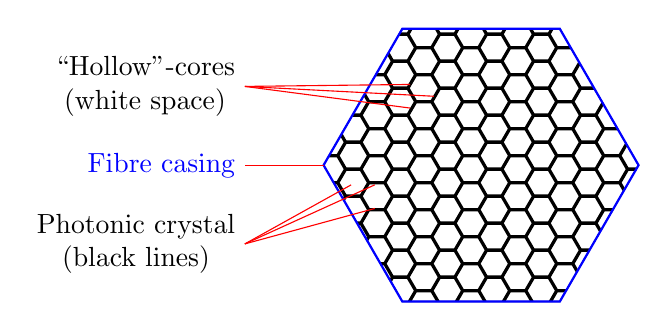
\begin{tikzpicture}
	%only need cross section plus labels
	
	%cross-section
	\begin{scope}[scale=1.0, shift={(0,0)}]
		\filldraw[pattern=hexagons] (0,0) -- (1,{sqrt(3)}) -- (3,{sqrt(3)}) -- (4,0) -- (3,{-sqrt(3)}) -- (1,-{sqrt(3)}) -- cycle;
		\draw[thick, blue] (0,0) -- (1,{sqrt(3)}) -- (3,{sqrt(3)}) -- (4,0) -- (3,{-sqrt(3)}) -- (1,-{sqrt(3)}) -- cycle;
	\end{scope}
	
	%labels for everything
	\draw[red] (0,0) -- (-1,-0);
	\node[anchor=east, color=blue] at (-1,0) {Fibre casing};
	\draw[red] (1.1,1.025) -- (-1,1);
	\draw[red] (1.1,0.725) -- (-1,1);
	\draw[red] (1.4,0.875) -- (-1,1);
	\node[anchor=east, align=center] at (-1,1) {``Hollow"-cores \\ (white space)};
	\draw[red] (0.65,-0.25) -- (-1,-1);
	\draw[red] (0.35,-0.25) -- (-1,-1);
	\draw[red] (0.65,-0.55) -- (-1,-1);
	\node[anchor=east, align=center] at (-1,-1) {Photonic crystal \\ (black lines)};

\end{tikzpicture}

\end{document}